
\documentclass[letterpaper,hide notes,xcolor={table,svgnames},pdftex,10pt]{beamer}
\def\showexamples{t}


%\usepackage[svgnames]{xcolor}

%% Demo talk
%\documentclass[letterpaper,notes=show]{beamer}

\usecolortheme{crane}
\setbeamertemplate{navigation symbols}{}

\usetheme{MyPittsburgh}
%\usetheme{Frankfurt}

%\usepackage{tipa}

\usepackage{hyperref}
\usepackage{graphicx,xspace}
\usepackage[normalem]{ulem}
\usepackage{multicol}

\newcommand\SF[1]{$\bigstar$\footnote{SF: #1}}

\usepackage[default]{sourcesanspro}
\usepackage[T1]{fontenc}

\newcounter{tmpnumSlide}
\newcounter{tmpnumNote}

% old question code
%\newcommand\question[1]{{$\bigstar$ \small \onlySlide{2}{#1}}}
% \newcommand\nquestion[1]{\ifdefined \presentationonly \textcircled{?} \fi \note{\par{\Large \textbf{?}} #1}}
% \newcommand\nanswer[1]{\note{\par{\Large \textbf{A}} #1}}


 \newcommand\mnote[1]{%
   \addtocounter{tmpnumSlide}{1}
   \ifdefined\showcues {~\tiny\fbox{\arabic{tmpnumSlide}}}\fi
   \note{\setlength{\parskip}{1ex}\addtocounter{tmpnumNote}{1}\textbf{\Large \arabic{tmpnumNote}:} {#1\par}}}

\newcommand\mmnote[1]{\note{\setlength{\parskip}{1ex}#1\par}}

%\newcommand\mnote[2][]{\ifdefined\handoutwithnotes {~\tiny\fbox{#1}}\fi
% \note{\setlength{\parskip}{1ex}\textbf{\Large #1:} #2\par}}

%\newcommand\mnote[2][]{{\tiny\fbox{#1}} \note{\setlength{\parskip}{1ex}\textbf{\Large #1:} #2\par}}

\newcommand\mquestion[2]{{~\color{red}\fbox{?}}\note{\setlength{\parskip}{1ex}\par{\Large \textbf{?}} #1} \note{\setlength{\parskip}{1ex}\par{\Large \textbf{A}} #2\par}\ifdefined \presentationonly \pause \fi}

\newcommand\blackboard[1]{%
\ifdefined   \showblackboard
  {#1}
  \else {\begin{center} \fbox{\colorbox{blue!30}{%
         \begin{minipage}{.95\linewidth}%
           \hspace{\stretch{1}} Some space intentionally left blank; done at the blackboard.%
         \end{minipage}}}\end{center}}%
         \fi%
}



%\newcommand\q{\tikz \node[thick,color=black,shape=circle]{?};}
%\newcommand\q{\ifdefined \presentationonly \textcircled{?} \fi}

\usepackage{listings}
\lstset{%
  keywordstyle=\bfseries,
  aboveskip=15pt,
  belowskip=15pt,
  captionpos=b,
  identifierstyle=\ttfamily,
  escapeinside={(*@}{@*)},
  stringstyle=\ttfamiliy,
  frame=lines,
  numbers=left, basicstyle=\scriptsize, numberstyle=\tiny, stepnumber=0, numbersep=2pt}

\usepackage{siunitx}
\newcommand\sius[1]{\num[group-separator = {,}]{#1}\si{\micro\second}}
\newcommand\sims[1]{\num[group-separator = {,}]{#1}\si{\milli\second}}
\newcommand\sins[1]{\num[group-separator = {,}]{#1}\si{\nano\second}}
\sisetup{group-separator = {,}, group-digits = true}

%% -------------------- tikz --------------------
\usepackage{tikz}
\usetikzlibrary{positioning}
\usetikzlibrary{arrows,backgrounds,automata,decorations.shapes,decorations.pathmorphing,decorations.markings,decorations.text}

\tikzstyle{place}=[circle,draw=blue!50,fill=blue!20,thick, inner sep=0pt,minimum size=6mm]
\tikzstyle{transition}=[rectangle,draw=black!50,fill=black!20,thick, inner sep=0pt,minimum size=4mm]

\tikzstyle{block}=[rectangle,draw=black, thick, inner sep=5pt]
\tikzstyle{bullet}=[circle,draw=black, fill=black, thin, inner sep=2pt]

\tikzstyle{pre}=[<-,shorten <=1pt,>=stealth',semithick]
\tikzstyle{post}=[->,shorten >=1pt,>=stealth',semithick]
\tikzstyle{bi}=[<->,shorten >=1pt,shorten <=1pt, >=stealth',semithick]

\tikzstyle{mut}=[-,>=stealth',semithick]

\tikzstyle{treereset}=[dashed,->, shorten >=1pt,>=stealth',thin]

\usepackage{ifmtarg}
\usepackage{xifthen}
\makeatletter
% new counter to now which frame it is within the sequence
\newcounter{multiframecounter}
% initialize buffer for previously used frame title
\gdef\lastframetitle{\textit{undefined}}
% new environment for a multi-frame
\newenvironment{multiframe}[1][]{%
\ifthenelse{\isempty{#1}}{%
% if no frame title was set via optional parameter,
% only increase sequence counter by 1
\addtocounter{multiframecounter}{1}%
}{%
% new frame title has been provided, thus
% reset sequence counter to 1 and buffer frame title for later use
\setcounter{multiframecounter}{1}%
\gdef\lastframetitle{#1}%
}%
% start conventional frame environment and
% automatically set frame title followed by sequence counter
\begin{frame}%
\frametitle{\lastframetitle~{\normalfont(\arabic{multiframecounter})}}%
}{%
\end{frame}%
}
\makeatother

\makeatletter
\newdimen\tu@tmpa%
\newdimen\ydiffl%
\newdimen\xdiffl%
\newcommand\ydiff[2]{%
    \coordinate (tmpnamea) at (#1);%
    \coordinate (tmpnameb) at (#2);%
    \pgfextracty{\tu@tmpa}{\pgfpointanchor{tmpnamea}{center}}%
    \pgfextracty{\ydiffl}{\pgfpointanchor{tmpnameb}{center}}%
    \advance\ydiffl by -\tu@tmpa%
}
\newcommand\xdiff[2]{%
    \coordinate (tmpnamea) at (#1);%
    \coordinate (tmpnameb) at (#2);%
    \pgfextractx{\tu@tmpa}{\pgfpointanchor{tmpnamea}{center}}%
    \pgfextractx{\xdiffl}{\pgfpointanchor{tmpnameb}{center}}%
    \advance\xdiffl by -\tu@tmpa%
}
\makeatother
\newcommand{\copyrightbox}[3][r]{%
\begin{tikzpicture}%
\node[inner sep=0pt,minimum size=2em](ciimage){#2};
\usefont{OT1}{phv}{n}{n}\fontsize{4}{4}\selectfont
\ydiff{ciimage.south}{ciimage.north}
\xdiff{ciimage.west}{ciimage.east}
\ifthenelse{\equal{#1}{r}}{%
\node[inner sep=0pt,right=1ex of ciimage.south east,anchor=north west,rotate=90]%
{\raggedleft\color{black!50}\parbox{\the\ydiffl}{\raggedright{}#3}};%
}{%
\ifthenelse{\equal{#1}{l}}{%
\node[inner sep=0pt,right=1ex of ciimage.south west,anchor=south west,rotate=90]%
{\raggedleft\color{black!50}\parbox{\the\ydiffl}{\raggedright{}#3}};%
}{%
\node[inner sep=0pt,below=1ex of ciimage.south west,anchor=north west]%
{\raggedleft\color{black!50}\parbox{\the\xdiffl}{\raggedright{}#3}};%
}
}
\end{tikzpicture}
}


%% --------------------

%\usepackage[excludeor]{everyhook}
%\PushPreHook{par}{\setbox0=\lastbox\llap{MUH}}\box0}

%\vspace*{\stretch{1}

%\setbox0=\lastbox \llap{\textbullet\enskip}\box0}

\setlength{\parskip}{\fill}

\newcommand\noskips{\setlength{\parskip}{1ex}}
\newcommand\doskips{\setlength{\parskip}{\fill}}

\newcommand\xx{\par\vspace*{\stretch{1}}\par}
\newcommand\xxs{\par\vspace*{2ex}\par}
\newcommand\tuple[1]{\langle #1 \rangle}
\newcommand\code[1]{{\sf \footnotesize #1}}
\newcommand\ex[1]{\uline{Example:} \ifdefined \presentationonly \pause \fi
  \ifdefined\showexamples#1\xspace\else{\uline{\hspace*{2cm}}}\fi}

\newcommand\ceil[1]{\lceil #1 \rceil}


\AtBeginSection[]
{
   \begin{frame}
       \frametitle{Outline}
       \tableofcontents[currentsection]
   \end{frame}
}



\pgfdeclarelayer{edgelayer}
\pgfdeclarelayer{nodelayer}
\pgfsetlayers{edgelayer,nodelayer,main}

\tikzstyle{none}=[inner sep=0pt]
\tikzstyle{rn}=[circle,fill=Red,draw=Black,line width=0.8 pt]
\tikzstyle{gn}=[circle,fill=Lime,draw=Black,line width=0.8 pt]
\tikzstyle{yn}=[circle,fill=Yellow,draw=Black,line width=0.8 pt]
\tikzstyle{empty}=[circle,fill=White,draw=Black]
\tikzstyle{bw} = [rectangle, draw, fill=blue!20, 
    text width=4em, text centered, rounded corners, minimum height=2em]
    
    \newcommand{\CcNote}[1]{% longname
	This work is licensed under the \textit{Creative Commons #1 3.0 License}.%
}
\newcommand{\CcImageBy}[1]{%
	\includegraphics[scale=#1]{creative_commons/cc_by_30.pdf}%
}
\newcommand{\CcImageSa}[1]{%
	\includegraphics[scale=#1]{creative_commons/cc_sa_30.pdf}%
}
\newcommand{\CcImageNc}[1]{%
	\includegraphics[scale=#1]{creative_commons/cc_nc_30.pdf}%
}
\newcommand{\CcGroupBySa}[2]{% zoom, gap
	\CcImageBy{#1}\hspace*{#2}\CcImageNc{#1}\hspace*{#2}\CcImageSa{#1}%
}
\newcommand{\CcLongnameByNcSa}{Attribution-NonCommercial-ShareAlike}

\newenvironment{changemargin}[1]{% 
  \begin{list}{}{% 
    \setlength{\topsep}{0pt}% 
    \setlength{\leftmargin}{#1}% 
    \setlength{\rightmargin}{1em}
    \setlength{\listparindent}{\parindent}% 
    \setlength{\itemindent}{\parindent}% 
    \setlength{\parsep}{\parskip}% 
  }% 
  \item[]}{\end{list}} 




\title{Lecture 3 --- The Canadian Legal System }

\author{Jeff Zarnett \\ \small \texttt{jzarnett@uwaterloo.ca}}
\institute{Department of Electrical and Computer Engineering \\
  University of Waterloo}
\date{\today}


\begin{document}

\begin{frame}
  \titlepage

\begin{center}
  \small{Acknowledgments: Douglas Harder~\cite{dwh}, Julie Vale~\cite{jv}}
  \end{center}
\end{frame}




\begin{frame}
\frametitle{The Canadian Legal System}

The Canadian Legal System is formed out of many traditions:

\begin{itemize}
	\item The Rule of Law
	\item Code Civil (in Qu\'ebec)
	\item English Common Law
\end{itemize}

\end{frame}



\begin{frame}
\frametitle{The Rule of Law}

As we've seen, it was once the case that monarchs were absolute.

Rulers claimed that they had the divine right to rule. 

They could make, and break, the law at a whim.

They were therefore above the law. 

\end{frame}



\begin{frame}
\frametitle{Judge Dredd}

\begin{center}
	
\includegraphics[width=0.3\textwidth]{images/dredd.jpg}
\end{center}

(Image and quote from the 1995 film.)

\end{frame}



\begin{frame}
\frametitle{Rule of Law}

The \alert{Rule of Law} is the principle that no-one is above the law.

Black's Law Dictionary defines it as:
\begin{quote}
The doctrine that every person is subject to the ordinary law within the jurisdiction.
\end{quote}

Rulers, even monarchs, are constrained by the law. 

The \textit{Oxford English Dictionary} defines it as:

\begin{quote}
The authority and influence of law in society, esp. when viewed as a constraint on individual and institutional behaviour; (hence) the principle whereby all members of a society (including those in government) are considered equally subject to publicly disclosed legal codes and processes.
\end{quote}

\end{frame}



\begin{frame}
\frametitle{Code Civil du Qu\'ebec}

Most jurisdictions in the world use the ``civil law'' system.

Civil codes contain a comprehensive statement of rules. 

The are often general principles to deal with any dispute that may arise.

In civil law cases, the judge considers only the application of the code to the case at hand.

Civil Law is used in the province of Qu\'ebec for provincial matters.\\
\quad This is for historical reasons from when it was a French colony.

\end{frame}



\begin{frame}
\frametitle{Common Law}

Canada, at a federal level, and in all other provinces, follows the common-law system as in England, the USA, and numerous other countries.

Medieval England had travelling judges who would render decisions.

One goal of the system was consistency: a similar legal case should produce a similar ruling.

Thus, when a case is heard, the ruling forms a \alert{precedent}.

The principle is \textit{stare decisis}: ``stand by decisions''.

Thus, courts should generally stand by the decisions previously made.\\
\quad This principle carries forward into the Canadian Legal System.

\end{frame}



\begin{frame}
\frametitle{Equity}

When it seemed that following the law would lead to an unfair result, subjects (litigants) could appeal to the King for \alert{equity}:

Equity, simply defined, is just \textit{fairness}.

A court may find that following a precedent leads to an unjust result, and may overturn a precedent on the basis of equity.

The idea of appeals still exists, though they are now to higher courts rather than to the Monarch...

\end{frame}



\begin{frame}
\frametitle{Common Law Today}

In addition to statutes and regulations, legal decisions made by judges are binding on judges below them.


This means there are three sources of law:
\begin{enumerate}
	\item Acts of the legislatures (e.g., Professional Engineers Act)
	\item Regulations, codes, by-laws, etc. (e.g., O. Reg. 941)
	\item Precedents set by previous judges (e.g., R v. Ron Engineering)
\end{enumerate}

\end{frame}



\begin{frame}
\frametitle{Precedent}

Thus, it is not enough to simply know the law and regulations...

It is also necessary to study previous cases in the area to understand the decisions and the reasoning.

Significant components of contract law are found only in precedent.

What if there is no precedent for the situation?

\end{frame}



\begin{frame}
\frametitle{Precedent}

Maybe there is a precedent that is ``close enough'' that can be applied?

Perhaps there is a precedent that is similar and can be modified?

Can we find a precedent from another common law country?\\
\quad The Supreme Court of New Zealand cites Canadian decisions quite often...

If there are no other sources, then a judge will have to set a new precedent.

\end{frame}



\begin{frame}
\frametitle{Precedent and Law}

As important as precedent is, parliament has supremacy.

That is to say, acts of Parliament (laws) supersede precedent. 

And parliament, of course establishes the court system and the rules of procedure in those courts.

\end{frame}



\begin{frame}
\frametitle{Lawsuits}

Recall that civil law is about restoring the injured party, to the extent possible, to its original state, or resolving a dispute between private parties.

If the parties cannot come to agreement without the intervention of the courts, a \alert{lawsuit} is the method to bring the court system into play.

The initiator of the legal action is the \alert{plaintiff}.

The plaintiff names in his or her complaint the party (parties) who has (have) allegedly wronged the plaintiff: the \alert{defendant(s)}.

The plaintiff must also specify the reason for the lawsuit: the \alert{cause of action}.

\end{frame}



\begin{frame}
\frametitle{Lawsuits}

A lawsuit, or \alert{case} will be heard by the courts in the form of a \alert{trial}.\\
\quad It may be a trial in front of a judge, or a jury.

Each side makes its case and introduces evidence to support its position.

Each side also has the opportunity to rebut the other side's case.

At any time before the ruling, the parties may come to an agreement outside the courts and \alert{settle} the matter without a need for the court to set terms.

\end{frame}



\begin{frame}
\frametitle{No-One Escapes Judgement}

Once the trial is concluded, the judge (or jury) will retire to consider the facts and arguments presented.

Unlike a criminal trial, the standard is not ``beyond a reasonable doubt'', but ``balance of probabilities''.

Thus, it is not necessary to prove one side's case to a certainty; only establish that one side's case is more likely than the other side's.


The judge (and possibly jury) will then deliver the \alert{judgement} or \alert{ruling}.\\
\quad This is the court's official finding of facts and awards of damages.



\end{frame}


\begin{frame}
\frametitle{The Judicial Structure}

\begin{center}
	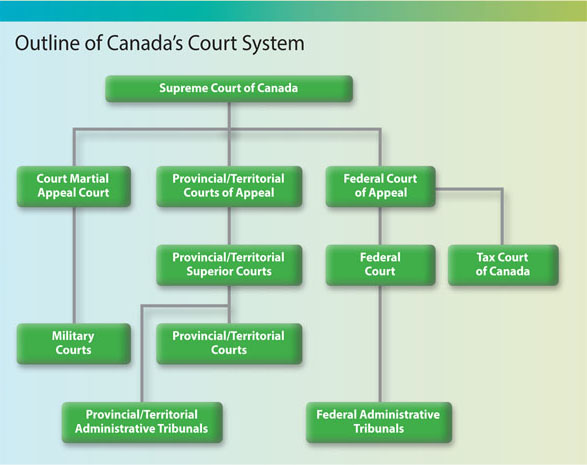
\includegraphics[width=0.8\textwidth]{images/courts.jpg}\\
	The Canadian Court System~\cite{just07}.
\end{center}

\end{frame}



\begin{frame}
\frametitle{Jurisdiction}

As we can see, there are many different courts in the country, each with different responsibilities.

Cases are initially heard in a ``lower'' court (at the bottom of the chart).

And the court must have \alert{jurisdiction} to hear the case.

One way to think of jurisdiction: authority to make a decision in the matter.

\end{frame}



\begin{frame}
\frametitle{Example of Jurisdiction}

The case of someone disputing his income tax assessment must be heard by the Tax Court of Canada.

If he attempted to file it in a military court or provincial court, the case would be dismissed or transferred because the court is not qualified to hear this case.

Similarly, if a contract is formed and executed in British Columbia, and a legal dispute arises, the case will be heard in B.C., not Nova Scotia...

We will return to the subject of jurisdiction later.

\end{frame}



\begin{frame}
\frametitle{The Courts}

Let us now examine the courts as described in the diagram.

The descriptions are from~\cite{just07}, as the government was kind enough to break it all down for us. 

We'll begin at the bottom and work our way up.

\end{frame}




\begin{frame}
\frametitle{Administrative Boards \& Tribunals}

These are an alternative way of resolving disputes.

They deal with application of laws and regulations, such as eligibility for disability benefits or human rights.

These are not strictly part of the court system, but their decisions are subject to judicial review.

\end{frame}



\begin{frame}
\frametitle{Provincial \& Territorial Courts}

Provincial courts try most criminal offences, money matters and family matters. 

The courts apply common-law principles (except in Qu\'ebec).

Provincial courts may also include specialized courts, such as youth courts, family courts, and small claims courts. 

Weird oddity: Nunavut has only one level of provincial court.

As before, at this level, the legal system in Qu\'ebec follows the civil code.

\end{frame}



\begin{frame}
\frametitle{Superior Courts}

Superior courts are the trial level of courts in a province or territory. 

They deal with the most serious criminal and civil cases and have the power to review the decisions of the provincial and territorial courts.

The trial level courts may be called the Supreme Court, the Court of Queen's Bench, or the Superior Court of Justice.

The appeal-level courts, or Courts of Appeal, hear civil and criminal appeals from the superior or provincial trial courts.

\end{frame}




\begin{frame}
\frametitle{Interruption: Court of Appeal}

Recall from earlier that in medieval England, a litigant could appeal to the King to have a ruling re-examined on the grounds of fairness. 

A similar idea exists in our legal system: a litigant may ask a higher court to review the decision made by a lower court.

It's not enough to simply be dissatisfied with the outcome; there must be a legal basis for this (called \alert{grounds for appeal})\footnote{And sometimes one must argue for the right to even file an appeal, seeking leave to appeal...}.

Appellate courts usually have the authority to decide whether to hear a case.\\
\quad If they think there is no legal issue to be examined, they will decline.

\end{frame}



\begin{frame}
\frametitle{Interruption: Court of Appeal}

An appeal is not a re-run of the original trial; it's a review by a panel of judges.

Lawyers may present arguments as to why the original trial was flawed or the ruling was inconsistent or unfair.

The purpose is not to re-examine the facts of the case.

The appellate court may rule to:

\begin{itemize}
	\item Uphold (affirm the decision of the lower court)
	\item Reverse (overrule the lower court)
	\item Vacate (annul the previous trial)
\end{itemize}

The court of appeal's decision need not be unanimous; a majority is adequate.

\end{frame}



\begin{frame}
\frametitle{Federal Courts}

The Federal Court specializes in areas such as intellectual property, maritime law, federal-provincial disputes, and civil cases related to terrorism.

The Tax Court specializes in hearing appeals from tax assessments.

The Federal Court of Appeal reviews the decisions of both these courts. 

In fact, it is the highest court of the land for about 95 percent of all cases.

\end{frame}

\begin{frame}
\frametitle{The Supreme Court}

The Supreme Court of Canada is the ultimate court of appeal. 

It hears appeals from decisions of the appeal courts in all the provinces and territories, as well as from the Federal Court of Appeal. 

Supreme Court judgments are final.

It decides important questions about the Constitution and controversial or complicated areas of private and public law. 

The government can also ask the Supreme Court for its opinion on important legal questions, such as senate reform.


\end{frame}



\begin{frame}
\frametitle{The Supreme Court}

Recall also that the Supreme Court is the interpreter of the constitution.

Its rulings on whether or not a law is constitutional are final.

The Supreme Court is, in a way, a check on the power of parliament.

\end{frame}



\begin{frame}
\frametitle{How It's Made: The Law}

We have discussed how courts interpret and apply the law, but where do laws come from?

Laws are acts of legislatures (parliament).

Legislative branches may have one or two bodies.\\
\quad One legislative body is called unicameral (one-chamber).\\
\quad Two is called bicameral (two-chambers).

A law is introduced and passed by the legislative assembly.

\end{frame}



\begin{frame}
\frametitle{Legislative Bodies}

In Canada, the federal legislature is bicameral.\\
\quad The House of Commons and the Senate.

Provincial/Territorial legislatures are unicameral.\\
\quad In Ontario, Provincial Parliament.\\
\quad In Qu\'ebec, the National Assembly.\\
\quad In most other provinces, House of Assembly or Legislative Assembly.

Once passed, a law needs \textit{royal assent}.

Royal assent is the monarch (or designated representative) signing the law.

\end{frame}


\begin{frame}
\frametitle{The Administration of Justice}

As we have seen, the government establishes the courts to administer justice and enforce the laws.

Judges are chosen from members of the legal profession.\\
\quad Those who are members of the \textit{Bar}.

Judges may not:
\begin{itemize}
	\item Engage in public debate about their decisions
	\item Express personal opinions on major social issues
	\item Engage in outside business
\end{itemize}

The judiciary is independent of the rest of the government (but judges are appointed by the government).

\end{frame}



\begin{frame}
\frametitle{Parliamentary Sovereignty}

Laws as passed by parliament are not subject to review... with one exception.

The courts may, as is specified in the constitution, rule on whether a law is constitutional: congruent with the constitution.

The courts do not decide whether a law is good or bad, or whether it needs amendment or repeal.

Remember: the constitution is the highest law of the land.

\end{frame}



\begin{frame}
\frametitle{Content of the Laws}

The content of the laws as passed will vary significantly.

Some laws are used to raise taxes (e.g., income tax) and spend money (e.g., purchase submarines for the Navy).

Others relate to criminal matters: forbidding stealing, or legalizing marijuana.

In both these categories, the government is involved somehow. 

\end{frame}



\begin{frame}
\frametitle{Content of the Laws}

Yet, a great deal of law is related to matters between parties, where neither one is a government of any sort.

For example, Alice makes a contract with Bob to buy a computer. 

Both Bob and Alice are private citizens, but the government does pass laws that regulate and dictate how Alice and Bob may interact in this transaction.

If, say, Bob has broken the contract, even though he may not have committed a crime, Alice may ask the courts to step in to hear the case and pass judgment...


\end{frame}


\begin{frame}
\frametitle{References \& Disclaimer}
\bibliographystyle{alphaurl}
\setbeamertemplate{bibliography item}{\insertbiblabel}
{\scriptsize
\bibliography{290}
}
\vfill

{\tiny Disclaimer: the material presented in these lectures slides is intended for use in the course ECE~290 at the University of Waterloo and should not be relied upon as legal advice. Any reliance on these course slides by any party for any other purpose are the responsibility of such parties.  The author(s) accept(s) no responsibility for damages, if any, suffered by any party as a result of decisions made or actions based on these course slides for any other purpose than that for which it was intended.\par}


\end{frame}


\end{document}

